\section{Automatic Overlay Customization} \label{sec:dse-framework}
A SCGRA overlay customization framework is proposed to
automatically adjust the overlay architecture to achieve 
better design trade-off for a specific compute intensive nested loop. 
A marginal performance revenue aware customization DSE is used to 
acquire a smaller feasible design space.
Within the feasible design space, customization for various design goals 
such as minimum energy consumption and minimum energy delay production can 
be obtained rapidly.

\subsection{Customization Framework}
\figref{fig:customization-framework} shows the proposed customization 
framework. It can be roughly divided into three steps including marginal performance 
revenue aware DSE, SCGRA overlay customization and SCGRA overlay compilation. 
The SCGRA overlay compilation with specified overlay configuration and loop 
transformation can be found in \secref{sec:background}, and we will mainly focus on the remaining 
two steps in this section.

\begin{figure}[H]
\center{\includegraphics[width=0.8\linewidth]{customization-framework}}
\caption{FPGA Accelerator Customization Framework}
\label{fig:customization-framework}
\end{figure}

The DSE is essentially used to determine the feasible design space. 
As presented in \figref{fig:customization-framework}, the DSE needs to 
go through the operation scheduling first to acquire the DFG performance.
Then the nested loop performance can be calculated with 
corresponding performance model. The detail of this model will be 
illustrated in next section. By comparing this configuration to previous acceptable configurations 
in the feasible design space, performance revenue can be obtained. 
If the revenue of a particular design parameter is lower than a 
pre-defined threshold, this configuration will be regarded as unacceptable. 
In addition, according to the observation in previous section, the 
configurations that are larger on this particular parameter will be set to be 
unacceptable as well because the marginal performance revenue decreases. 
Finally, these unacceptable configurations can be safely pruned and thus saves the
scheduling and estimation efforts. Similarly, overhead constraints can also be 
used to prune the design space. The configurations that are accepted 
will be added to the feasible design space. Overhead as well as performance 
of each feasible configuration will be stored and they can be used for 
further customization in the next step.

After the DSE, customization for various design goals such as energy 
consumption and energy delay production will start. It basically acquires 
these design goals through corresponding models and then search for 
the optimal design and configuration. 

Finally, customized overlay configuration and loop transformation 
options will be passed to the overly compilation step. The nested 
loop can be then compiled to FPGA bitstream and CPU binary code 
targeting the hybrid CPU-FPGA computation system.

\subsection{Performance Revenue Aware DSE}
The proposed performance revenue aware DSE algorithm 
is formalized and detailed in this section. 
Suppose $\bm{\Psi}$ represents the accelerator design 
space of a nested loop. $\bm{C}=(C_0, C_1, ..., C_N) \in \bm{\Psi}$ 
represents a possible configuration of the nested loop 
acceleration. $C_i$ stands for the $i$th design parameter 
of the configuration $\bm{C}$ and $C_i \in (C_i^0, C_i^1, ..., C_i^{R_i})$
where $R_i$ stands for the maximum No. of possible $C_i$.
$\bm{C}(i,j)=(C_0, C_1, ..., C_i^j,...)$ denotes a configuration 
in which the $i$th design parameter adopts the $j$th possible option. 
$\epsilon$ is the performance revenue metric and $\Phi$ denotes the 
feasible design space.

The algorithm is illustrated in \algref{alg:revenue}. 
It is essentially a brute-force search with online 
design space pruning using marginal performance revenue. 
As different design parameters may influence with each other, 
the marginal performance revenue is merely analyzed between 
two configuration vectors that differ on a single dimension of the 
vectors and it can be calculated by \eqref{eq:revenue}.

\begin{equation} \label{eq:revenue}
    \begin{split}
        Revenue(i,k)=1-\frac{LoopExeTime(\bm{C}(i,k+1))}{LoopExeTime(\bm{C}(i,k))} \\
    \end{split}
\end{equation}

In addition, there may be minor fluctuation due to the complex 
heuristics used in the operation scheduling. For example, 
larger SCGRA size may result in worse performance as displayed in 
\figref{fig:perf-influence}. This may mislead the design 
space pruning. To cope with this problem, multiple consecutive performance 
revenue should be evaluated as presented in this algorithm.

\begin{algorithm}[H]
\caption{Revenue Aware Design Space Exploration.}
\label{alg:revenue}
\begin{algorithmic}
\PROCEDURE{}
\STATE Init $State[\bm{C}]$ as False
\FORALL {$\bm{C} \in \bm{\Psi} \land (\neg State[\bm{C}])$} 
\STATE $i=1$
\WHILE {$i < N$}
\STATE $k$ is integer such that $C_i==C_i^k$
\STATE Perform simulation with configuration $\bm{C}(i,k)$
\STATE Estimate performance $LoopExeTime(\bm{C}(i,k))$
\STATE Estimate overhead $Overhead(\bm{C}(i,k))$
\IF {$Revenue(i, k-1)>\epsilon \lor Revenue(i, k)>\epsilon$}
\STATE Add $\bm{C}(i,k)$ to $\bm{\Phi}$
\STATE Set $State[\bm{C}]$ as True
\ELSE 
\STATE $j=k$
\WHILE {$j<=R_i$}
\STATE Set $State[\bm{C}]$ as True
\ENDWHILE
\ENDIF
\STATE $i=i+1$
\ENDWHILE
\ENDFOR
\ENDPROCEDURE
\end{algorithmic}
\end{algorithm}

\subsection{Performance and Overhead Models}
In this section, we will mainly explain the performance and 
hardware overhead models which will be used for both the design 
space exploration and customization. 

\subsubsection{Performance Model}
In order to map the nested loop to an SCGRA overlay, the loop will 
be partially unrolled and the unrolled part will be transformed to a 
DFG. Then the DFG will be scheduled to the overlay. In order to 
improve the transmission efficiency, a few identical 
DFGs will be further grouped and each group needs only a single IO 
transmission. 

Suppose each group consists of $DFGPerGroup$ DFGs 
and the nested loop contains $GroupPerLoop$ groups.
$DFGExeTime$ denotes the execution time of a DFG 
which can be acquired from the operation scheduler.
The execution time of the loop which includes both the 
computation time and the communication time can be 
calculated by \eqref{eq:loopexetime}. We use DMA for the 
communication between the SCGRA overlay and host CPU and the DMA 
can be estimated using a piece wise linear modeled function 
denoted by $DMALat(x)$ where $x$ stands for the amount of 
data to be transmitted. Then the communication can be 
calculated by \eqref{eq:comm}.

\begin{equation} \label{eq:loopexetime}
    \begin{split}
        LoopExeTime=&GroupPerLoop \times DFGPerGroup \\
                    &\times DFGExeTime + CommTime
    \end{split}
\end{equation}

\begin{equation} \label{eq:comm}
\begin{split}
    CommTime=&(DMA(GroupIn) + DMA(GroupOut)) \\
             &\times GroupPerLoop
\end{split}
\end{equation}

\subsubsection{Overhead, Power and Energy Models}
FPGA hardware overhead mainly involves DSP, LUT, FF and 
RAM block. DSP and RAM block consumption can be calculated directly 
with specified overlay configuration while LUT and FF are 
estimated through a linear model of SCGRA size. 

Power consumption is consisted of RAM block power, 
clock power, signal power, DSP power and so on. 
We notice that the BRAM power consumption has better linearity 
with the amount of BRAM consumption while the rest part of the power 
is linear to the SCGRA size. Thus the power consumption can 
be calculated by \eqref{eq:power} where $\alpha$ and $\beta$ 
are linear model coefficients.

\begin{equation}\label{eq:power}
\begin{split}
	Power=&RAMOverhead \times RAMUnitPower \\
	      &+ \alpha \times SCGRASize + \beta
\end{split}
\end{equation}

With the performance and power models, we can further acquire the energy
consumption model which is the production of power and loop execution time 
and energy power delay product model which is the production of energy 
consumption and loop execution time.

